\section{Motivation and thesis overview}
\label{sec:motivation}
This section presents the primary motivation for this thesis and provides an overview of its structure.

A key objective in robotics is to develop autonomous robots that can perform a wide range of manipulation tasks, such as pick-and-place and assembly operations, in response to specific commands. These tasks often involve varying degrees of freedom, like object categories, for a specific task there can different objects of interest, and positions, the initial state of the environment (how and where the object are arranged) is not fixed.

In traditional industrial settings, manually coded control rules are effective for managing situations where robots follow fixed and repetitive paths. This is possible because the categories and positions of objects are known in advance, and the robot workspace remains constant over time (e.g., the workcell shown in Figure \ref{fig:industrial_robots_example}).

However, the modern landscape of social robotics and contemporary industrial applications requires a higher level of \textbf{adaptability} and \textbf{flexibility}. Robots are now expected to operate in environments shared with human operators, receiving commands and interacting with them in a collaborative or cooperative manner. For example, a robot may be tasked with picking up a tool and delivering it to an operator. This requires the robot to not only recognize different object categories and estimate their positions but also to correlate the outcomes of environmental analysis with the commands received, adapting its actions accordingly to exhibit ``intelligent'' behaviors.

\begin{figure}[htb]
    \centering
    %\begin{subfigure}[b]{0.6\textwidth}
    %    \centering
    %    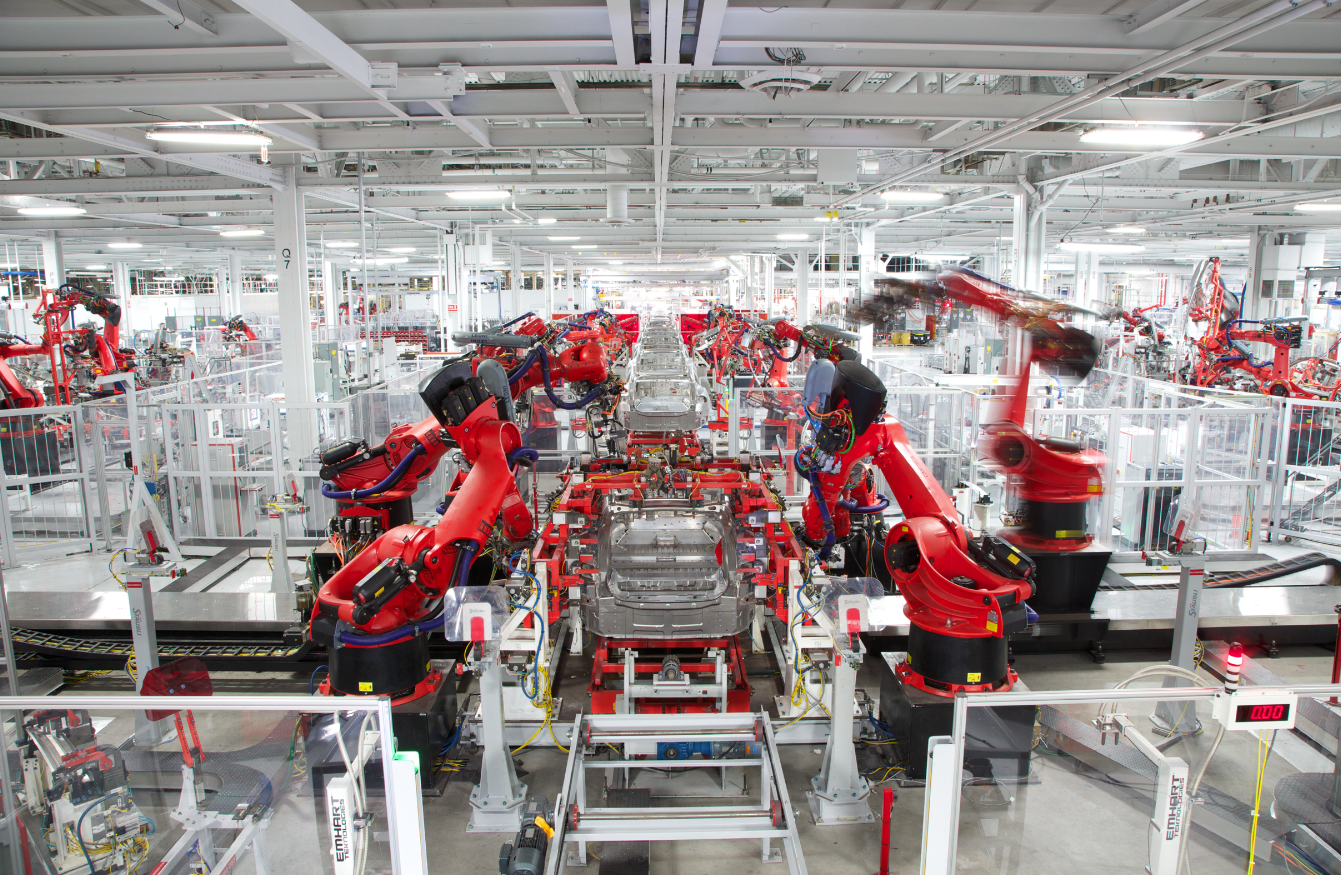
\includegraphics[width=\textwidth]{Figures/images/assembly.jpg}
    %    \caption{Robots involved in Tesla Assembly line}
    %    \label{fig:assembly}
    %\end{subfigure}
    %\hfill
    \begin{subfigure}[b]{0.45\textwidth}
        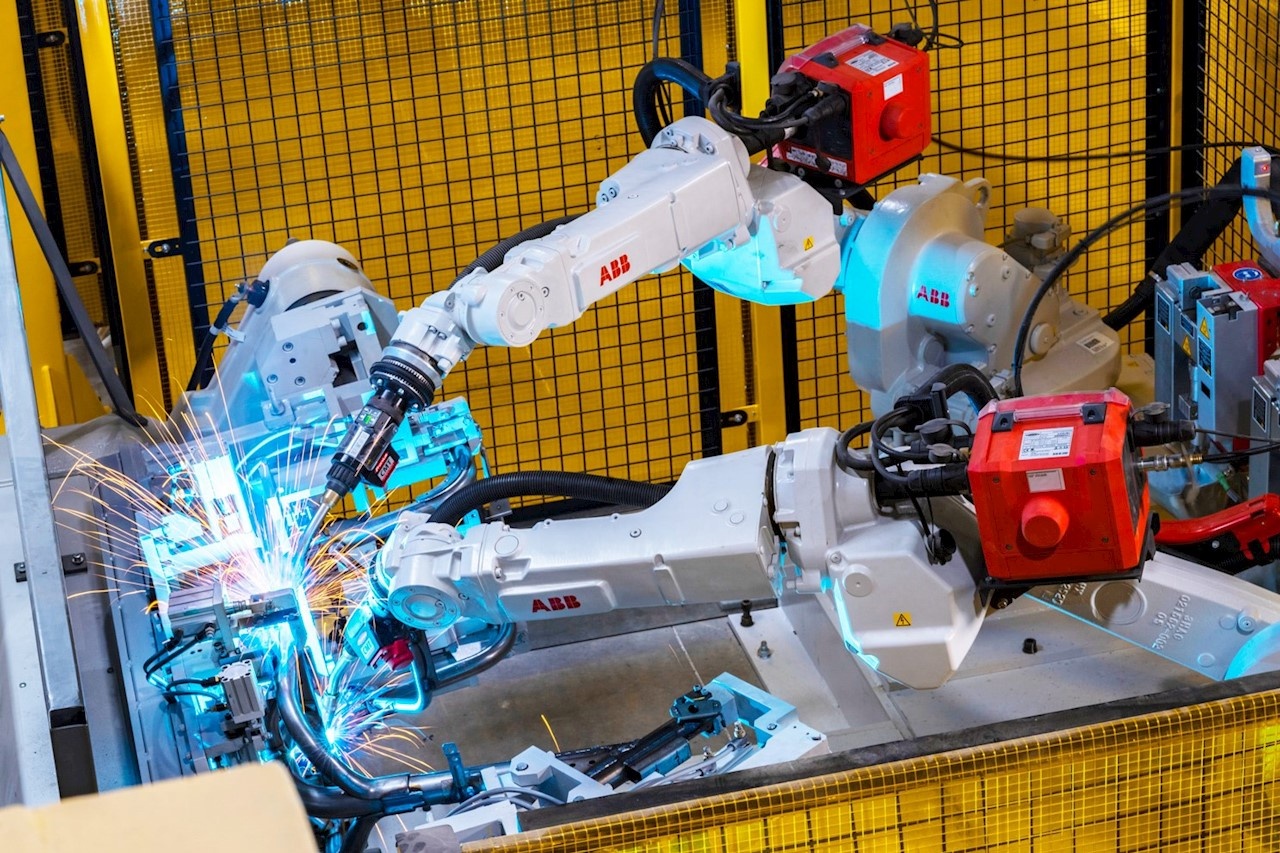
\includegraphics[width=\textwidth]{figures/images/welding.jpg}
        \caption{Robots involved in arc welding operation.}
        \label{fig:welding}
    \end{subfigure}
    \hfill
    \begin{subfigure}[b]{0.5\textwidth}
        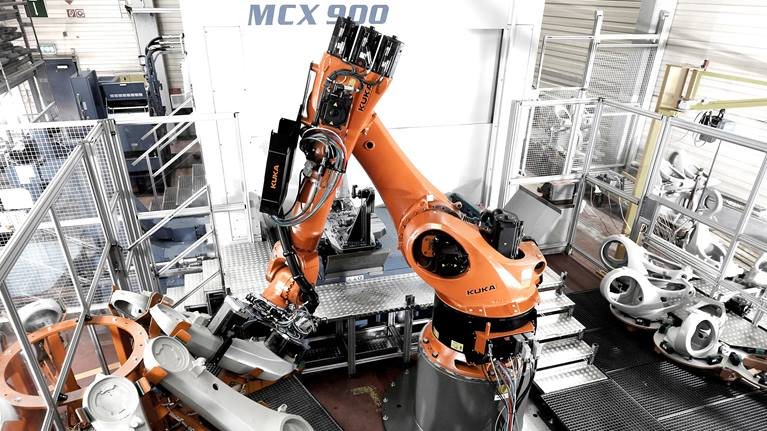
\includegraphics[width=\textwidth]{figures/images/loading.jpg}
        \caption{Robot involved in loading operation.}
        %\vspace{0.5cm}
        \label{fig:material_handling}
    \end{subfigure}
   \hfill
   \caption{Industrial Robots: example of applications.}
   \label{fig:industrial_robots_example}
\end{figure}



To address this problem, the scientific community has focused on evaluating the use of \textit{data-driven} approaches. These methods include Imitation Learning algorithms, which leverage data from examples of desired behaviors, often referred to as demonstrations, to enable a robot to replicate the demonstrated tasks.

Multi-Task Imitation Learning methods, as highlighted in \cite{jang2022bc_z, dasari2021transformers_one_shot, mandi2022towards_more_generalizable_one_shot, brohan2022rt}, are particularly promising due to their ability to meet the requirements of both high adaptability and flexibility. These methods use a \textbf{multi-task dataset}, which contains demonstrations for $n$ different tasks (e.g., pick-and-place, nut-assembly, etc.), to fit a \textit{single control function} denoted as $\pi^{L}_{\theta}(a_{t}|s_{t}, c_{m_{i}})$. This function maps the current observed state $s_{t}$ and the command $c_{m_{i}}$ into the corresponding action $a_{t}$ to be executed by a physical robot. The command $c_{m_{i}}$ refers to the $m^{th}$ variation of the $i^{th}$ task (e.g., the pick-and-place task can have different variations based on the target object and the target placing spot).

While these methods have shown significant potential, challenges remain in both single-task and multi-task scenarios. As reported in \cite{jang2022bc_z, yu2018daml}, existing systems struggle with identifying critical task points, such as determining when to close the gripper near an object or when to open it near the placement area, rather than understanding the broader intent of the task. Moreover, performance drops occur when scenes involve distractor objects, i.e., objects that do not contribute to task execution. This underscores the need for enhanced capabilities to correctly correlate commands with the results of scene analysis to identify target objects.

In the context presented so far, this thesis addresses the problem of \textit{Visual-Conditioned Multi-Task Imitation Learning}. The goal is to develop a system that can advance the realization of a \textit{versatile collaborative robot} suitable for industrial applications. This robot should be capable of executing tasks directed by a human operator and acquiring new skills based on a limited number of demonstrations, building upon its existing knowledge. To illustrate potential applications, consider a collaborative workspace where a human operator could instruct the robot to provide a tool or engage in assembly tasks. Specifically, the focus is on exploring methods that rely on \textit{visual inputs}, where the current state $s_{t}$ is an image depicting the robot's workspace, and the command $c_{m_{i}}$ is given in terms of video demonstrations of an agent (e.g., robot or human) executing the desired task.

This thesis addresses the problem of Visual-Conditioned Multi-Task Imitation Learning from a different perspective. Current state-of-the-art methods typically address this challenge using end-to-end architectures trained with an action-centric behavioral cloning loss. In these methods, the system receives high-level inputs (such as images of a task demonstration and the agent current observation) and generates corresponding low-level control actions.

However, in scenarios involving multiple tasks or variations of tasks, manipulation contains both control and cognitive problems. Specifically, two main challenges must be addressed:

\begin{enumerate}
    \item \textbf{Command Analysis and Understanding}: The first challenge is analyzing the given command. From a high-level task command, the system needs to understand the \textbf{intent} (e.g., picking and placing versus assembling), identify the relevant objects (e.g., selecting the blue box instead of the red one), and recognize the required skill (e.g., reaching, following, or picking).

    \item \textbf{Action Generation}: The second challenge is correlating features from the observed state with the information derived from the command. The goal is to create an intermediate representation that integrates relevant information from both inputs (e.g., focusing on the portion of the image containing the target object). This representation should highlight key details necessary for inferring the correct action based on both the current state and the command.
\end{enumerate}

Addressing these challenges with end-to-end architectures is particularly difficult, especially in scenes with multiple similar objects that could either be distractors or the actual object of interest depending on the task. Indeed, as shown by preliminary results and evaluation of state-of-the-art methods, there is a recurring issue of \textbf{target object misidentification}. While these methods can produce control policies that result in smooth and reasonable behaviors for high-level tasks like pick-and-place or nut-assembly, they often manipulate the wrong object, failing to complete the task correctly.

To address this issue, this thesis proposes an approach that explicitly tackles the two challenges described before, introducing modular architectures, rather than end-to-end systems. These modular architectures are composed of modules that are specifically designed to handle the tasks of command analysis and understanding, as well as action generation.

Specifically, this approach tries to leverage the well-known capabilities of deep architectures in solving problems like object detection to introduce \textbf{object priors}. These object priors can provide crucial information to the control system about the regions of interest in the workspace where objects of interest are located, thereby improving the \textbf{robustness} of the system against distractor objects as well as the \textbf{interpretability} of the system, since the cognitive module can return information about the region of the image where the robot is intended to move.

In conclusion, this thesis is organized as follows. Section \ref{sec:sota} presents an overview of the classic methods used to address the Learning from Demonstration problem. Chapter \ref{ch:cod} introduces the Conditioned Object Detection module, designed to solve the cognitive aspect of the decision-making problem. Chapter \ref{ch:occp} presents the Object Conditioned Control Policy, aimed at solving the control aspect of the decision-making problem. Chapter \ref{ch:real_world_application} details the validation of these methods in a real-world scenario. Finally, Section \ref{sec:conclusion} provides a summary of the results and discusses potential future research directions.

% \smalltodo{Continue with organization, after prof ack.}
% The observed results can be explained through a comprehensive analysis of the underlying learning procedure. Specifically, the reference methods \cite{dasari2021transformers_one_shot,mandi2022towards_more_generalizable_one_shot,brohan2022rt} propose end-to-end architectures that starting from \textbf{high-level inputs} (e.g., images and text) directly generate the required action, assuming that there is an implicit solution to the initial challenges associated with the command analysis and comprehension. These architectures are trained based on the principles of Behavioral Cloning (BC). BC offers two main approaches: one involves minimizing the disparity between the predicted and correct actions (as shown in Formula \ref{eq:mse}), while the other centers on maximizing the likelihood of executing the correct action (as shown in Formula \ref{eq:nll}). The choice between these approaches hinges on the nature of the policy, whether deterministic or probabilistic. It's important to note that all of these loss functions primarily target the predicted action, directly addressing step 2, with an implicit assumption of resolving step 1. This approach has exhibited effectiveness in simple scenarios where the robot has to learn a single task without variations \cite{zhang2018deep_vr_teleoperation,duan2017one_shot_il} and in multi-task settings where scenes are comprised of easily distinguishable objects \cite{dasari2021transformers_one_shot,mandi2022towards_more_generalizable_one_shot,brohan2022rt}. However, in complex scenarios composed of different distractor objects, the cognitive task becomes considerably more intricate and may be beyond resolution solely through the information derived from the action-based loss, increasing the gap that exists between the training metric and the actual goal (i.e., understand the command, genarete the action based on the current state and the command comprehension, and solve the desired task).
% Starting from all the considerations above, the stated problem can be faced in two ways:
% \begin{enumerate*}[label=(\arabic*)]
%     \item Enhancing dataset diversity by expanding the representation of objects and employing a large-scale model capable of assimilating all the knowledge inherent in the dataset.
%     \item Dividing the Decision-Making Problem into two primary blocks, namely a reasoning module and an action module. This segmentation enables the independent validation of each task within the decision-making process and the separate evaluation of the performance of each block. Subsequently, a method should be devised to integrate these two components, creating a modular system capable of solving complex problems. This system would consist of interconnected modules designed to address simpler problems.
% \end{enumerate*}

% This thesis is situated within the context of Learning from Demonstration for robotic manipulation tasks. The objective is to develop a control function that can guide a robotic system to perform manipulation tasks by mimicking behaviors observed in expert demonstrations. Unlike traditional LfD methods that typically train a task-specific control function, this thesis tackles a more challenging problem known as Multi-Task Imitation Learning. Inspired by the way humans can solve various tasks simply by observing others, the goal here is to create a control policy capable of addressing multiple variations of a given task as well as entirely different tasks, all based on visual demonstrations of another agent performing the required tasks.

% This thesis approaches the problem of Visual-Conditioned Multi-Task Imitation Learning from a different perspective. Indeed, current state-of-the-art methods typically address this issue using end-to-end architectures, which are trained with an action-centric behavioral cloning loss. This means that, given high-level inputs (e.g., images of a task demonstration and the current observation of the agent), the system must generate the corresponding low-level control actions. However, in a scenario involving multiple tasks or multiple variations of a task, manipulation is not just a control problem but also a cognitive one. The system must understand the intent behind the demonstration and identify objects of interest within the current scene. This task is particularly challenging when the scene includes multiple similar objects, which could either be distractors or objects of interest depending on the specific task. Indeed, as showed in preliminary results and state-of-the-art methods evaluations, a problem of \textbf{target object missindenfication} has been observed. Obtaining control policy that are able to solve the control task in a correct way, since they produce smooth and reasonable behaviors of the robot solving the high-level requested task (pick-place, nut-assembly and so on), but manipulating most of the time the wrong object. 

% For this reason, starting from all the observation above, this thesis address the problem by a different perspective, solving explictly the cognitive task behind the decision making problem.

